\documentclass[runningheads,a4paper]{llncs}

\usepackage{amssymb}
\setcounter{tocdepth}{3}
\usepackage{graphicx}
\usepackage{subfig}
%\linespread{2}

\usepackage{url}
\usepackage{csquotes}
\newcommand{\keywords}[1]{\par\addvspace\baselineskip
\noindent\keywordname\enspace\ignorespaces#1}

\usepackage{listings}
\usepackage{color}
\usepackage{enumitem}
\usepackage{hyperref}

\definecolor{dkgreen}{rgb}{0,0.6,0}
\definecolor{gray}{rgb}{0.5,0.5,0.5}
\definecolor{mauve}{rgb}{0.58,0,0.82}

\lstset{frame=tb,
  language=C++,
  aboveskip=3mm,
  belowskip=3mm,
  showstringspaces=false,
  columns=flexible,
  basicstyle={\small\ttfamily},
  numbers=left,
  numberstyle=\tiny\color{gray},
  keywordstyle=\color{blue},
  morekeywords={vector},
  commentstyle=\color{dkgreen},
  stringstyle=\color{mauve},
  breaklines=true,
  breakatwhitespace=true,
  tabsize=3
}

\begin{document}

\mainmatter  % start of an individual contribution

% first the title is needed
\title{c3particles: \\ Modeling a Particle System in C++}

% a short form should be given in case it is too long for the running head
\titlerunning{c3particles}

%
\author{Rosalie Kletzander}
%
\authorrunning{c3particles}
% (feature abused for this document to repeat the title also on left hand pages)

\institute{Practical Course "Advanced Software Development with Modern C++"\\Summer Term 2018\\Institute for Computer Science\\
Ludwig-Maximilians-Universit\"at M\"unchen\\
}

\maketitle


%\begin{abstract}
%
%
%%keywords{network operating systems, programmable networks, Software-Defined Networking, SDN-controllers}
%\end{abstract}

\section{Introduction}
Particle systems are used in many different areas: most prominently in the entertainment industry in games and movies and for simulations and visualizations scientific research. No matter the area of application, the basic rules governing these systems are the same: the laws of physics. c3particles (cpp particles) implements a model of a particle system in C++ that separates the physical concepts and laws from the underlying graphics library. This enables a mathematical formulation of the forces influencing the particles.


\section{Short Recap of Physics}

In order to be able to model the physics of a particle system, it is necessary to first understand the basic rules of motion.

Newton's First Law of Motion states:
\begin{quotation}
Every object in a state of uniform motion tends to remain in that state of motion unless an external force is applied to it.
\end{quotation}

This means that an object will not move unless it is accelerated by a force, which brings us to Newton's Second Law of Motion:
\begin{quotation}
The relationship between an object's mass \emph{m}, its acceleration \emph{a}, and the applied force \emph{F} is $ F = m*a $.
\end{quotation}

With this information it is possible to calculate the acceleration of an object by dividing the applied force by the object's mass. The next step is deriving the velocity and location of the object per time step by integration.

The velocity of an object can be calculated by integrating the acceleration over time t. 
\begin{equation}
\overrightarrow{v}(t) = \int \mathrm{(\overrightarrow{a})} \mathrm{d}t = \overrightarrow{a}*t + C_v
\label{eq:vel}
\end{equation}

C is the integration constant, in this case it is equal to the velocity of t-1 for discrete time steps. Integrating the velocity over t yields the location.

\begin{equation}
\overrightarrow{s}(t) = \int \mathrm{(\overrightarrow{v})} \mathrm{d}t = \int (\overrightarrow{a}*t + C_v) \mathrm{d}t = \frac{\overrightarrow{a}*t^2}{2} + C_s
\label{eq:loc}
\end{equation}

Analogous to $C_v$, $C_s$ is equal to the location at t-1.

These formulas serve as the foundations of the physical model of the particle system. 

\section{Modeling the Particle System}
In order to model a particle system, it is necessary to understand the different underlying concepts.

%\begin{itemize}
%\item elements of the system: particle (newtonian object)
%\item force
%\item particle is passive, it doesn't "care" where the force is coming from $\rightarrow$ need some way to apply a force to a particle
%\item update at each time step
%\end{itemize}

\subsection{Concepts}
A particle system is actually a fairly simple construct. It contains objects, its "particles", which are understood to be objects that behave according to newtonian physics, i.e. "newtonian objects". They have a location, velocity, acceleration and mass. According to Newton's laws, an object will not change its motion unless it is accelerated by a \emph{force}. As a result, it is necessary to have the concept of a force.

In fact, these two concepts, "newtonian object" and "force" are sufficient for modeling a particle system. The basic .. expressions ..:

\paragraph{Particle $\ll$ Force}
applies a force to a particle using the formulas \ref{eq:vel} and \ref{eq:loc}

\paragraph{Force calc\_force(Particle, Particle, Function)}
calculates a force between two particles using the supplied function, when given the same particle twice, it returns the additive identity

\paragraph{Force gravity(Particle, Particle, List params)}
a specialization of calc\_force for calculating the gravitational force between two particles (is not actually a concept, but shows what calc\_force is capable of)

\paragraph{Force accumulate(Particle, ParticleContainer, Function)}
calc\_force for p with each other p in the container and reduce (addition) to one force

\paragraph{Force accumulate(Particle, ParticleContainer, List params, Function)}
use a pre-defined function to calculate the forces, pass initializer list for parameters

paragraph{Force accumulate(List forces)}
sum up a set of forces

\subsection{Time}
\begin{itemize}
\item discrete time steps
\item each time step (frame) triggers a new set of calculations
\end{itemize}

%examples why it is cool: reverse, 

\section{Implementation}

c3particles contains several separate modules (Figure~\ref{fig:sysdia}. The Particle System module contains the physical model and uses input given by the user to select forces. It updates the particles that are then read by the Particle Renderer, which uses the location to calculate the vertices and faces that need to be drawn. It passes the vertex buffers of all the particles to the OpenGL Rendering Pipeline, which processes them accordingly. It then writes the framebuffer to the screen and triggers a new calculation.

%\begin{itemize}
%\item system diagram

%\item for each time step (signaled by OpenGL), the Particle System module calculates the new values for all the particles based on the input given by the user control window. These values are then read by the Particle Renderer and used to fill the vertex buffers depending on the visualization selected (e.g as points or cubes)
%\item then, the OpenGL Rendering Pipeline renders the frame, using the provided shaders
%\item as soon as the screenbuffer is swapped, the calculation for the next frame is started
%\end{itemize}

\textbf{
\begin{figure}[]
\centering
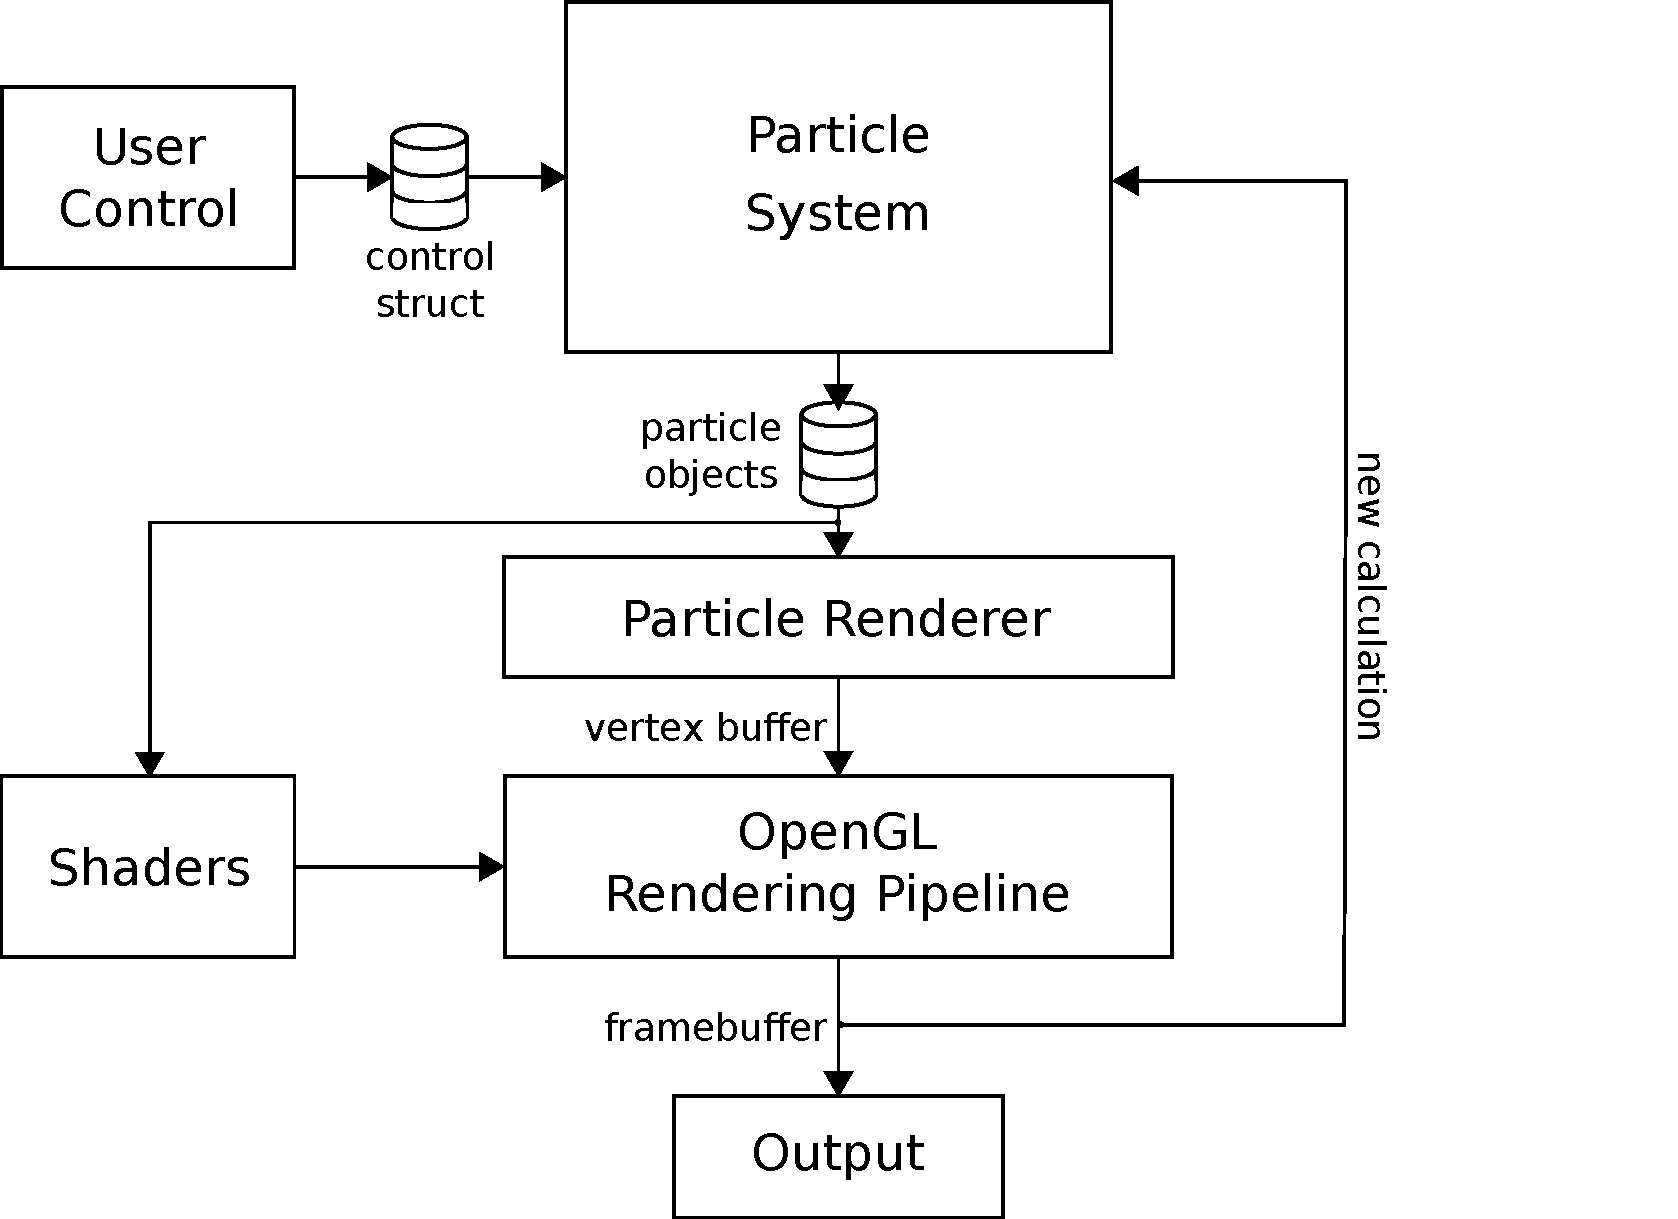
\includegraphics[width=0.8\textwidth]{images/system-diagram.pdf}
\caption{c3particles system diagram}
\label{fig:sysdia}
\end{figure}
}

\subsection{Particle System}
The Particle System module contains the physical model of the particle system and the particle objects (Figure~\ref{fig:sysdiadetail})
The physical model contains algorithms for calculating the forces on the particles, and the particles themselves. For each frame, the old values of the particles are read and used to update to the new values. The functions used to update the values are taken directly from \ref{eq:vel} \ref{eq:loc}

\textbf{
\begin{figure}[]
\centering
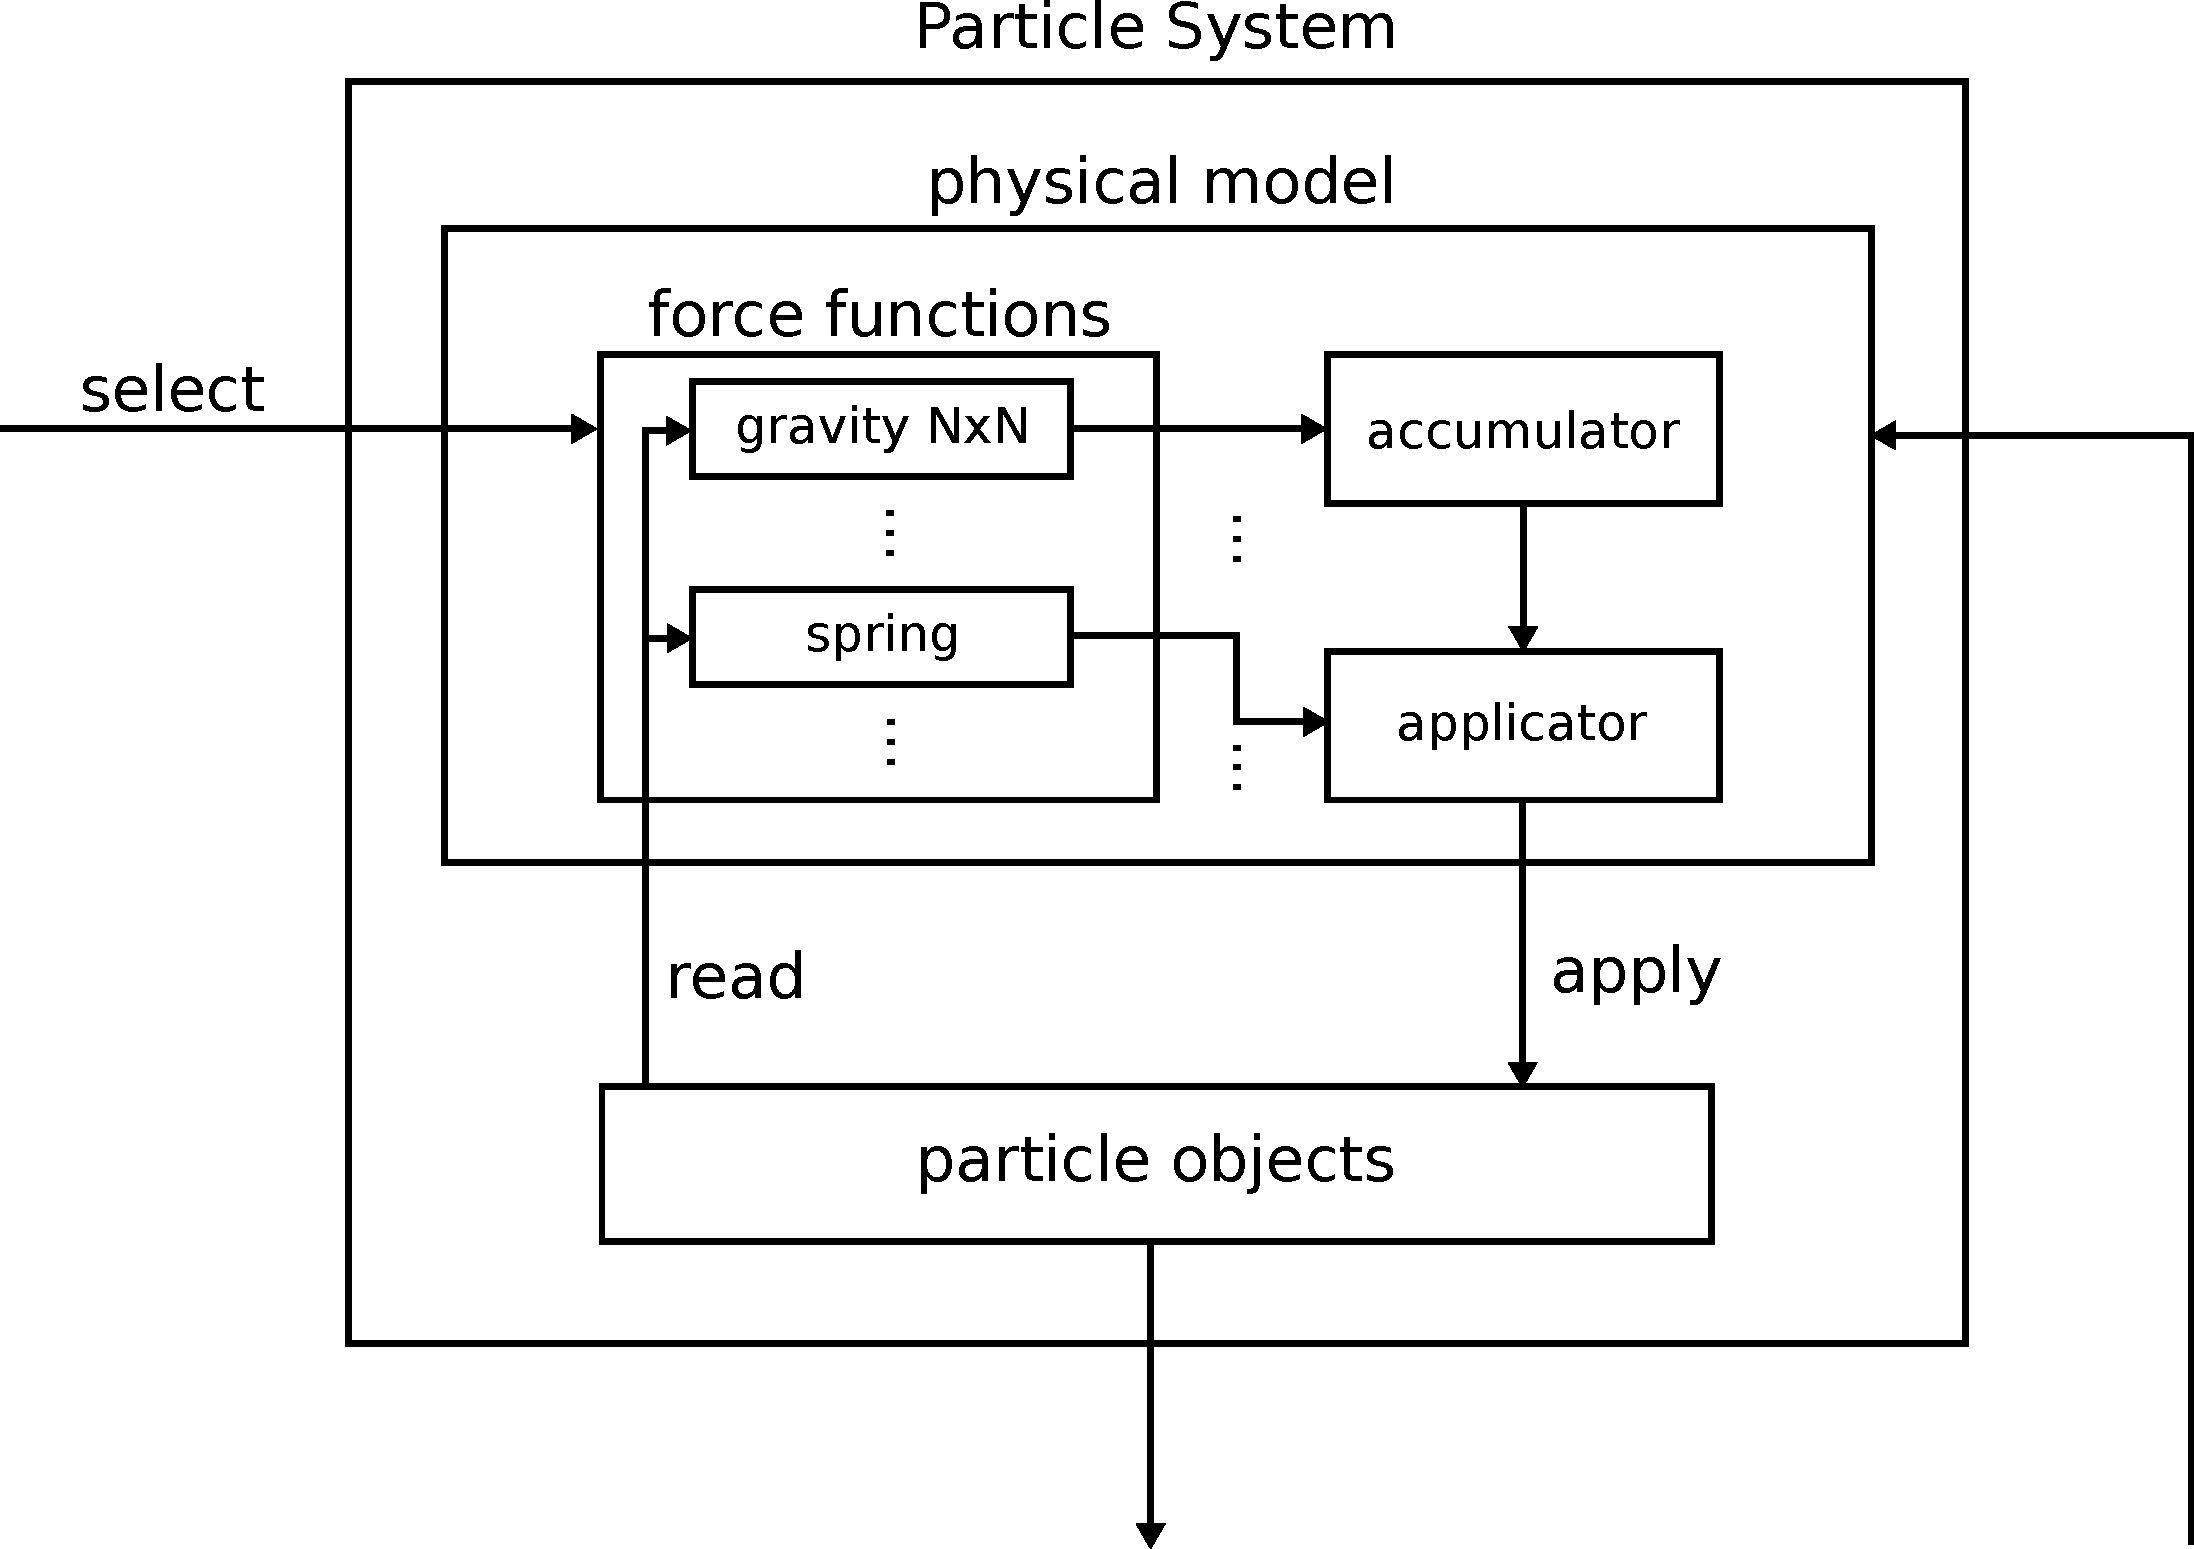
\includegraphics[width=0.8\textwidth]{images/particle-system-detail.pdf}
\caption{detailed diagram of the particle system}
\label{fig:sysdiadetail}
\end{figure}
}

\begin{figure}[tb]
\begin{lstlisting}
void ParticleSystem::update()                                                              
{                                                                                          
  // deltaT will always be 1.0 because calculation is based on frames                               
  for (Particle &p : _particles)                                                           
    {                                                                                      
      //v(t) = a*t + v(t-1)                                                            
      p.velocity = p.acceleration * 1.0f + p.velocity; //deltaT = 1.0                                  
                                                                                           
      //s(t) = (a*t^2)/2 + v(t) + s(t-1)                                               
      p.location = (p.acceleration * 1.0f) / 2.0f + p.velocity + p.location;
                                       	
      //acceleration is not accumulative, but recalculated at each time step          
      p.acceleration = {0, 0, 0};
    }                                                                                      
}                                                            
\end{lstlisting}
 \caption{ParticleSystem::update()}
 \label{fig:update}
\end{figure}

\subsubsection{Algorithms}
\begin{itemize}
\item concepts and expressions come to fruition here
\item differentiation between "external" forces and inter-particle forces
\item apply force $"<<"$
\item calc\_force
\item accumulate
\item specializations of calc\_force, e.g. gravity
\end{itemize}

The concepts and expressions defined above are incorporated into the system's algorithms. For the calculation of the forces it is helpful to split them logically into "inter-particle forces" and "external forces". The former refers to the forces that exist between all pairs of particles (e.g. gravitational forces) and the latter refers to forces that are applied to each particle independently of all others (e.g. wind).



\subsubsection{Particle Container}
The particles need to be stored in some data structure. At the moment, this is a std::vector which provides all the needed operations.

\subsection{User Control Window}
The user controls are implemented with gtk. The control window runs in a different thread that fills a C struct with the values set by the user. These values are then read by the system in order to calculate the desired forces.

\subsection{Particle Renderer}
The particle renderer iterates over the particles in the particle system and fills the vertex buffers for each one. How the vertex buffers are filled depends on the function called. At the moment, it is possible to render the particles as pixels with no depth perception and uniform size (\emph{c3p::ParticleRenderer::renderPoints}
or as cubes (\emph{c3p::ParticleRenderer::renderCubes}). The size of the cubes depends on the size of the particle (which, at the moment is dependent on its mass). The vertex buffers are then passed to the OpenGL Rendering Pipeline.

\subsection{Shaders}

\subsection{Graphics Engine}
The graphics engine is only secondary for this project. OpenGL was chosen because of its wide-spread use, however, with an appropriate particle renderer, any one could be used.

\subsection{Optimization}
\begin{itemize}
\item force matrix? 
\item parallelize particle calculation (works very well, because applyforce only updates acceleration, so location and velocity are unchanged until all forces have been calculated)
\end{itemize}

\section{Future Work}
\begin{itemize}
\item binary space partitioning
\end{itemize}



\bibliography{literature}
\bibliographystyle{plain}

\end{document}
